\chapter{Řídící SW}

Řídící software pro osazovací automat byla nejtěžší část celého projektu. SW spojuje jednotlivé části popsané v předcházejících kapitolách do jednoho celku. 



Jeden z hlavních požadavků na řídící SW byla jeho platformová nezávislost. Tedy možnost spuštění aplikace jak na operačním systému Linux, tak i na Windows. Protože aplikace má grafické rozhraní, zúžil se výběr mnou známých programovacích jazyků na C/C++, Java, Delphi a Python. Byl vybrán  právě poslední zmiňovaný Python, jelikož má velice dobrou dokumentaci a nástroje pro tvorbu GUI jsou uživatelsky přívětivé.
Tato kombinace slibovala rychlý prototyping SW a naději na funkční SW. Pro tvorbu GUI padla volba na PyQt.

V aplikaci je kvůli centrování součástek a desek potřebné i vyhodnocování obrazu. Jako základ byla použita hojně používaná knihovna OpenCV. Ta nabízí set základních funkcí pro manipulaci s obrazem. Implementované funkce jako rozostření, hledání hran, kontur a kruhů zjednoduší úlohu rozpoznávání pozice a rotace součástek a hledání centrovacích bodů DPS.


Screenshoty z QTGUI a pár věcí ohledně PyQt
\begin{figure}[h!]
  \centering
    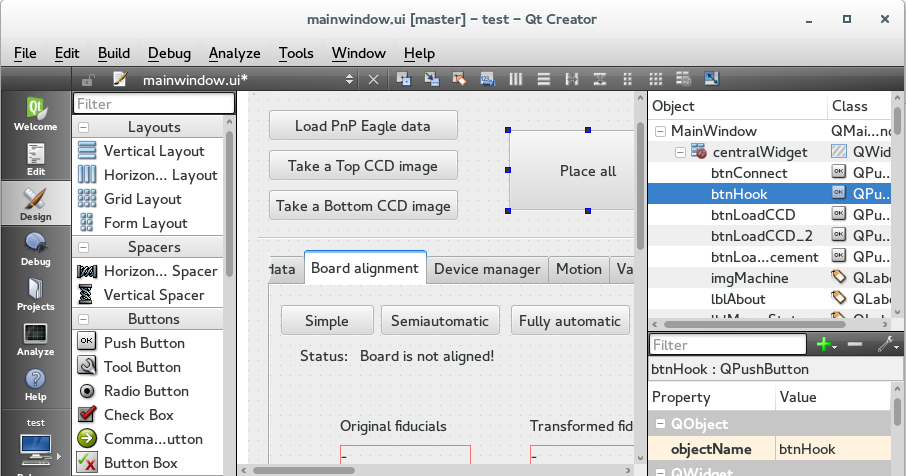
\includegraphics[width=1\linewidth]{obrazky/pyqt.png}%
    \caption{Vývojové prostředí PyQt pro tvorbu grafického rozhraní.}
\end{figure}







\section{Data pro osazovací automat}

Pro návrh elektronických systémů se používá software spadající do kategorie EDA – Electronic Design Automation. Je to soubor nástrojů pro tvorbu desek plošných spojů (a integrovaných obvodů). Mezi základní nástroje patří Schématické editory, simulátory obvodů, autoroutery, návrhové prostředí pro tvorbu DPS a CAM procesor. 
Příkladem EDA softwérů jsou: Altium Designer, KiCad, CadSoft Eagle.

Pro testování byl použit poslední zmiňovaný CadSoft Eagle, který je ve své základní varianě pro nekomerční účely dostupný zdarma. Uvžujme vytvořené schéma a DPS. Pro osazovací automat potřebujeme získat pozici, hodnotu, typ pouzdra a rotaci každé SMD součástky, dále potřebujeme získat pozici centrovacích značek. K tomu se částečně dají použít jendak vestavěné funkce, Eagle ale disponuje i možností použití tzv ULP (User Language Program. ) skriptů. ULP je programovací jazyk postavený na základech C a umožňuje přímé modifikování schématu, DPS a vytváření různých exportů.


Vestavěný export
Jednou z cest jak vyexportovat pozice součástek je \verb|File->Export->Partlist|


Výsledný export obsahuje všechny použité součástky a exportované pozice jsou v jednotkách mil. Pro osazovací automat je ale potřeba jen SMD součástek a centrovacích bodů. Tento export tedy není příliš vhodný, protože by potřeboval ještě následnou ruční úpravu spočívající minimálně v odmazání všech THD součástek


\begin{table}[h!]
  \caption{Ukázka exportu. }
  \begin{center}
  	\small
	  \begin{tabular}{|c|c|c|c|c|c|}
	    \hline
	    Part	& Value 	& Package 	& Library 	& Position (mil) 	& orientation	\\
	    \hline\hline

		C1 	& .1uF		& C0603		& resistor	& (2860 300)		& R180		\\
		\hline
		C2 	& 18pF		& C0603		& rcl		& (2075 1405)		& R90		\\
		\hline
	    \hline
	  \end{tabular}
  \end{center}
\end{table}

Součástí instalace Eagle je i několik již připravených ULP skriptů pro export, například Centroid\_ScreamingCircuits\_smd.ulp
Ten generuje oproti Partlistu strojově čitelnější formát a exportuje jen SMD součástky. Bohužel však chybí typ použitého pouzdra a hodnota součástky. 

\begin{verbatim}
  RefDes,Layer,LocationX,LocationY,Rotation
  C1,Top,2.860,0.300,180
  C2,Top,2.075,1.405,90
\end{verbatim}

Pro vytvoření exportu se všemi potřebnými hodnotami tak bylo potřeba napsat vlastní ULP skrip. 
Ten exportuje středy/origins součástek tak, jak byly vytvořené autorem součástky v knihovnách, dále i geomterické středy součástek. Geomterický střed funguje tak, že se iteruje nad všemi ploškami součástky a hledá se minimum a maximum v obou osách. Jejich rozdíl se vydělí dvěma a najde se skutečný střed součástky. Není to tak střed součástky základě geometrického tvaru pouzdra! Na to je třeba brát později zřetel. Důvod pro export těchto souřadnic je ten, že né všechny součástky v knihovnách se drží zažitého standardu na umisťování středícího bodu do středu pouzdra, případně do levého horního rohu.

Ukázka z ULP skriptu exportující informace o centrovacích bodech DPS

\begin{verbatim}
  printf("Part name;Package;Value;X origin;Y origin;\n");
  printf("%%fiducials\n");
  B.elements(E) if (E.populate) {

    if (E.package.name == "FIDUCIAL_1MM") 
         printf("%s;%s;%s;%.3f;%.3f;\n",
         E.name, E.package.name, E.value, u2mm(E.x), u2mm(E.y));  


  }
  printf("%%end_fiducials\n");
\end{verbatim}

Výsledný export je pak ve formátu 
\begin{verbatim}
  %data
  Part name;X center;Y center;X origin;Y origin;Rotation;Value;Package
  C1;72.644;7.620;72.644;7.620;180;.1uF;C0603
  C2;52.705;35.687;52.705;35.687;90;18pF;C0603
  %data_end
  %fiducials
  Part name;Package;Value;X origin;Y origin;
  U$3;FIDUCIAL_1MM;FIDUCIAL;7.500;3.000;
  U$4;FIDUCIAL_1MM;FIDUCIAL;7.500;57.000;
  U$6;FIDUCIAL_1MM;FIDUCIAL;92.500;3.000;
  %fiducials_end
\end{verbatim}

skript také exportuje obrázek dané DPS, který se dá po načtení do řídícího SW použít pro simulaci osazování. Celý skript je přiložen v příloze B.



\section{Workflow}

\begin{figure}[h!]
  \centering
    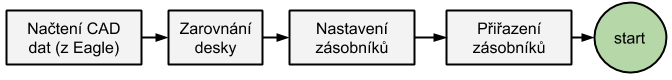
\includegraphics[width=1\linewidth]{obrazky/workflow.png}%
    \caption{Workflow.}
\end{figure}

\section{Program}

Mimo grafické rozhraní je součástí aplikace i terminál, ve kterém jsou logovány prováděné operace. Do terminálu se vypisují i návratové hodnoty z jednotlivých funkcí programu, hodí se tak pro odhalování případných problémů s aplikací.


\begin{figure}[h!]
  \centering
    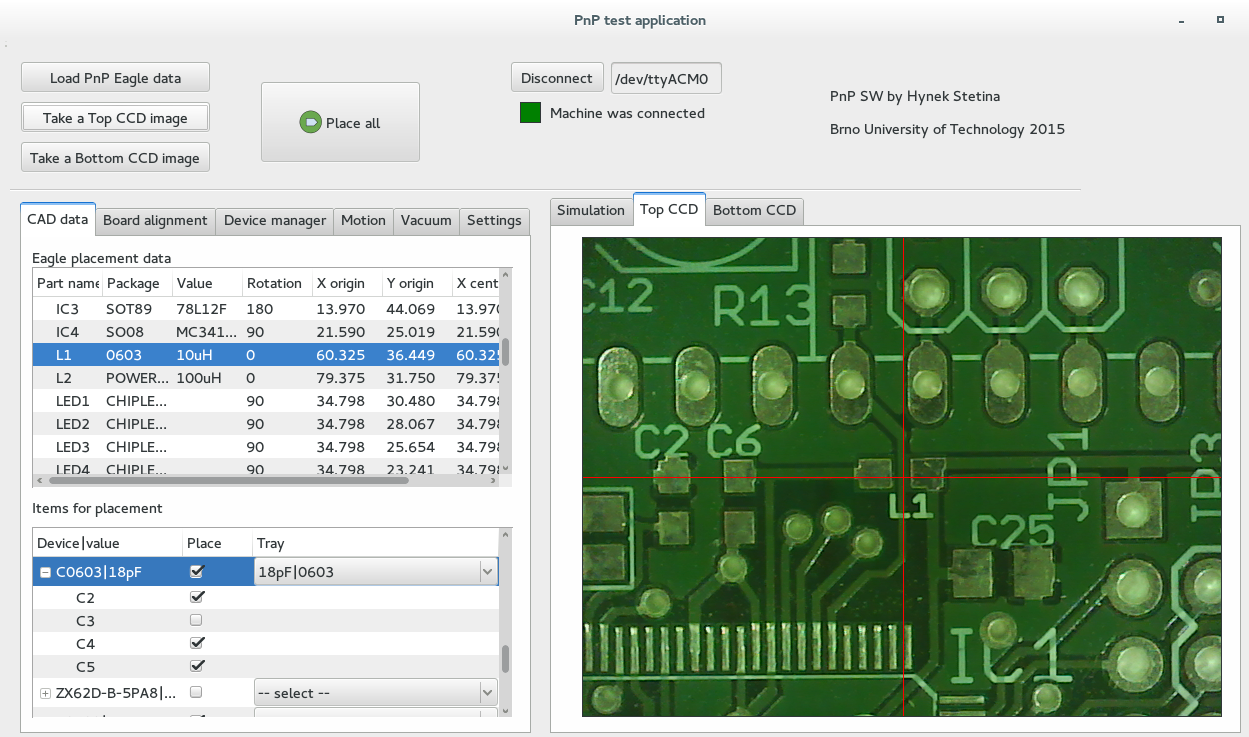
\includegraphics[width=1\linewidth]{obrazky/sw.png}%
    \caption{Hlavní obrazovka řídícího SW.}
\end{figure}


\subsection{CAD data a přiřazení zásobniků}
Po načtení CAD dat vyexportovaných z Eagle (tlačítko Load PnP data) jsou všechny součástky vylistovány do tabulky placement data. U každé položky v tabulce jsou uvedeny všechny potřebné data k jejímu osazení. Navíc pokud je již zarovnaná DPS, pomocí dvojkliku myší automat dojede s kamerou nad místo, kde má být součástka osazena a automaticky vytvoří náhledový snímek z horní CCD kamery.
Součástky stejného druhu (pouzdro|hodnota) jsou sdruženy v tabulce Items for palacement. U každého druhu součástek se zde přiřazuje příslušný zásobník, ze kterého budou součástky odebírány. Pomocí checkboxů lze volit, jestli bude daná součástka, nebo cellá skupina součástek osazována. Jak je vidět na obrázku, kondenzátor C3 nebude tak osazen.
\begin{figure}[h!]
  \centering
    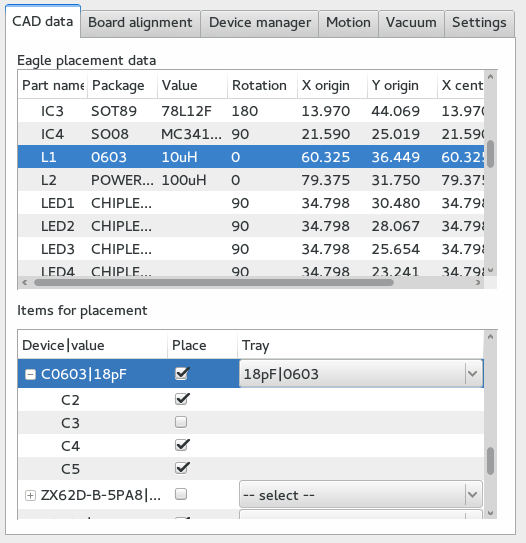
\includegraphics[width=0.6\linewidth]{obrazky/sw7.png}%
    \caption{Tabulka všech součástek a sdružené součástky podle pouzder a hodnoty.}
\end{figure}

\subsection{Zaměření DPS}
Pro přesné zaměření pozice DPS byly implementovány 3 centrovací algoritmy. V průběhu výroby DPS můžou vznikat různé chyby, které se ve výsledku porojeví v přesnosti osazování. Může se jednat o chybu měřítka, rotaci motivu vůči fyzickým rozměrům DPS a další. Obzvlášť znatelné jsou tyto chyby při podomácku vytvářených DPS. Další chyby můžou nastat při nepřesném uložení DPS do osazovacího automatu.

Základním zaměřovacím algoritmem je mód Simple - ten nepoužívá zádné vyhodnocování obrazu. DPS se umístí na dorazy, kdy jeden z jejích rohů je v souřadnici 0,0 (v souřadnicovém systému v prostoru pro DPS, ne v souřadnicovém systému celého stroje). Tato metoda je nejméně přesná, protože není schopna kompenzovat žádné chyby. Přesnost osazování v tomto módu tak závisí na preciznosti vycentrování DPS a její kvalitě.
jediná výhoda tohot módu je možnost osazovat i DPS, které nedisponují centrovacími značkami.

Nejužitečnější je plně automatický mód, který centruje DPS pomocí centrovacích značek (viz kapitola o vyhodnocování obrazu). Dokáže tak kompenzovat všechny výše popsané chyby. DPS je stejně jak v předchozím případě umístěna rohem do pozice 0,0. Princip spočívá v tom, že automat postupně najíždí nad centrovací značky a zjišťuje jejich skutečnou pozici vůči souřadnicovému systému automatu. Poté jsou všechny souřadnice součástek na DPS transformovány do nového souřadnicového systému. 

Posledním centrovací metodou je poloautomatický mód. Ten umožňuje zaměření DPS libovolně umístěné v pracovním prostoru. Má všechny výhody plně automatického módu jen s počáteční nutností najet nad každou z centrovacích značek ručně.

TODO, obrázek s naznačením jednotlivých metod.


\begin{figure}[h!]
  \centering
    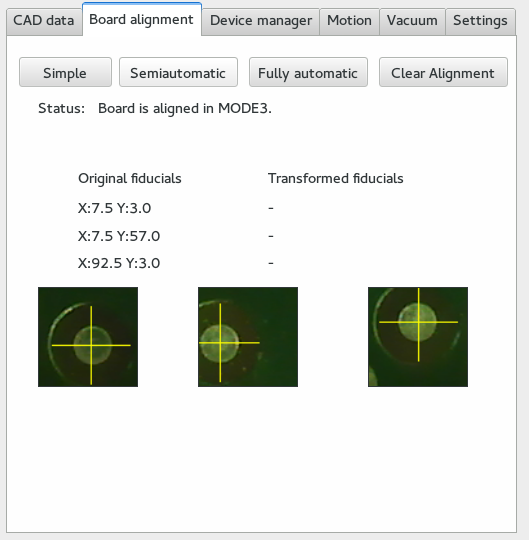
\includegraphics[width=0.6\linewidth]{obrazky/sw4.png}%
    \caption{Záložka s centrováním DPS.}
\end{figure}

\subsection{Manažer zásobníků}

V manažeru zásobníků je monžné vytvážet a editovat jednotlivé zásobníky. V průběhu psaní diplomové práce byla implementována jen možnost statického zásobníku\cite{fig:xxx}, SW je ale připraven pro různé typy zásobníků jako plata a tuby. statický zásobník má následující možosti nastavení:

\begin{itemize}
\item Rozteč součástek v pásce - parametr P1 z obrázku  \cite{fig:tape2}
\item Orientace pásky - jakým směrem jsou orientovány součástky vůči první referenční součástce
\item Počet součástek na pásce
\item Index aktuální součástky - inkrementuje se po každé odebrané součástce
\item Použít vyhodnocování obrazu - kontrola přítomnosti součástky na základě metody z SW XXXX
\item Vacuum test - Kontrola přítomnosti součástky na základě metody z VACUUM XXXX
\end{itemize}

Po nastavení těchto parametrů je potřeba zaměřit první součástku v zásobníků pomocí kamery a uložit tlačítkem Save. V tuto chvíli je zásobník připraven k použití.

\begin{figure}[h!]
	\centering
	\begin{subfigure}[b]{0.48\linewidth}
		\centering
		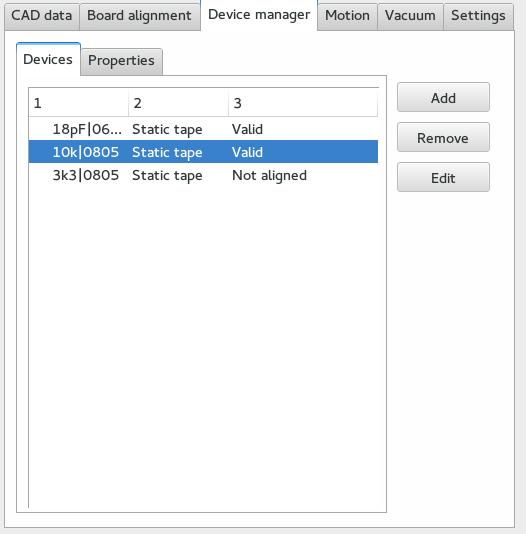
\includegraphics[width=1\linewidth]{obrazky/sw3.png}%
		\caption{AAAA.}
		\label{fig:denni}
	\end{subfigure}
	~
	\begin{subfigure}[b]{0.48\linewidth}
		\centering
		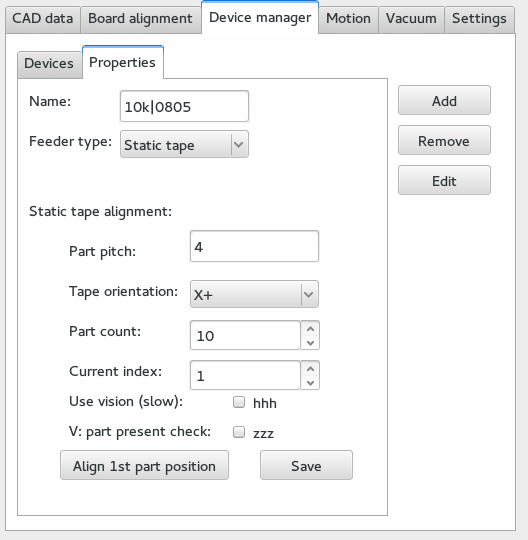
\includegraphics[width=1\linewidth]{obrazky/sw2.png}%
		\caption{BBBB.}
		\label{fig:denni2}
	\end{subfigure}

	\caption{Manažer zásobníků.}
\end{figure}


\subsection{Ovládání pohybu automatu}
Pro manuální pohyb s osazovací hlavou slouží záložka motion. Pomocí šipek tak lze pohybovat s hlavou po krocích 0.1mm, 1mm a 10mm. V ose Z je krok 1mm a pro rotaci byl implementován krok 1 STUPEŇ.
Tlačítko 0 automaticky nastaví kameru na souřadnici 0,0 v pracovním prostoru pro DPS.

Součástí této záložky jsou i skripty na měření přesnosti a reprodukovatelnosti.
\begin{figure}[h!]
  \centering
    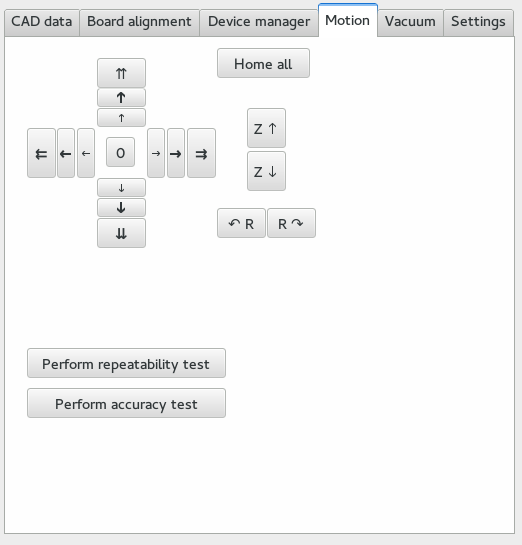
\includegraphics[width=0.6\linewidth]{obrazky/sw5.png}%
    \caption{Motion záložka.}
\end{figure}


\subsection{Vacuum}
Záložka pro monitorování aktuálního stavu tlaku v potrubí. Pomocí tlačítek Open/Close valve lze manuálně ovládat vakuový ventil. 
\begin{figure}[h!]
  \centering
    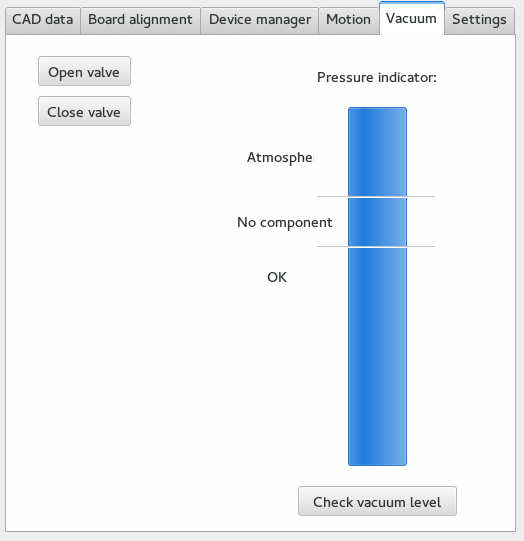
\includegraphics[width=0.6\linewidth]{obrazky/sw6.png}%
    \caption{Vacuum záložka.}
\end{figure}
 
